\begin{figure}[t]
  \centering
  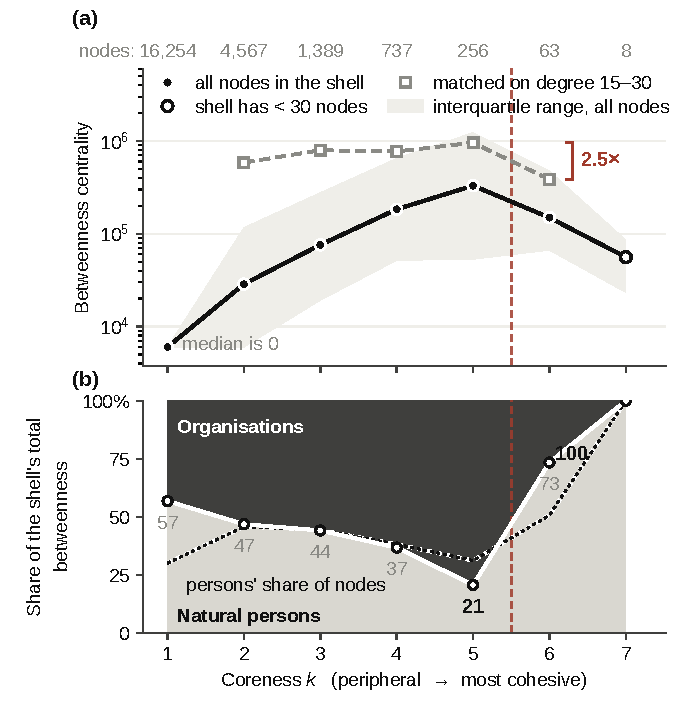
\includegraphics[width=\textwidth]{fig14_cohesion_brokerage.pdf}
  \caption{\textbf{Brokerage is non-monotonic in cohesion.}
  Panel (a): betweenness centrality by $k$-core shell, median with
  interquartile range shaded. Brokerage rises to a peak at $k$=5
  and falls in the more cohesive shells inside it. The dashed series repeats
  the comparison among nodes of comparable degree
  (15--30 ties), where the median falls from
  957,498 at $k$=5 to
  384,446 at $k$=6, a factor of
  2.5; the fall is therefore
  not a degree artefact. Panel (b): the composition of each shell's
  brokerage inverts at the same boundary. Organisations hold
  79\% of betweenness at
  $k$=5 and 27\% at
  $k$=6. The dotted line gives natural persons' share of each
  shell's \emph{nodes}, so the two can be compared: persons are
  31\% of the $k$=5 shell
  but hold only 21\% of its brokerage,
  and 51\% of the $k$=6 shell
  while holding 73\% of its brokerage. The
  inversion is therefore not a headcount effect. At $k$=7 the
  shell consists of 8 natural persons and no organisation at
  all, so its 100\% is compositional and is reported as description
  only.
  Cells of fewer than 30 nodes are drawn with open markers and excluded from
  the degree-matched series; the $k$=7 shell holds 8
  nodes and is descriptive only.
  $N = 23,274$ entities in the largest connected component.}
  \label{fig:cohesion-brokerage}
\end{figure}
